\section{Background and related work}
As the background knowledge to this work, we present a quick review of Convolution Neural Network (CNN) and transfer learning. Then we discuss relevant literature for object detection followed by quick discussion on background subtraction techniques. 


\subsection{Convolutional Neural Network (CNN)}
CNN based architectures are the most widely used models for solving computer vision based tasks such as image classification, object detection and object segmentation. During the last few years, they have proved their effectiveness in solving many image based problems. In a normal feed-forward neural network, input must be vectorized and each input feature is connected to each output feature in each layer. This results in huge number of parameters. Further, due to vectorization, the image loses its spacial structure and features computed by subsequent neural network layers can not be mapped to image coordinates. CNN by design avoids both of these problems. It not only uses far less no. of parameters than traditional feed-forward network but also preserves the 2D grid based structure of image\cite{arkar_thesis}.

Due to fast pace research in this domain, many new architectures have been proposed. However, convolution layer, pooling layer and fully connected layer still are the most widely used components of any CNN based architecture. Figure \ref{fig:lenet-5} shows architecture of one of the earliest CNN network which employed all three above mentioned basic components. 

\begin{figure}
    \centering
    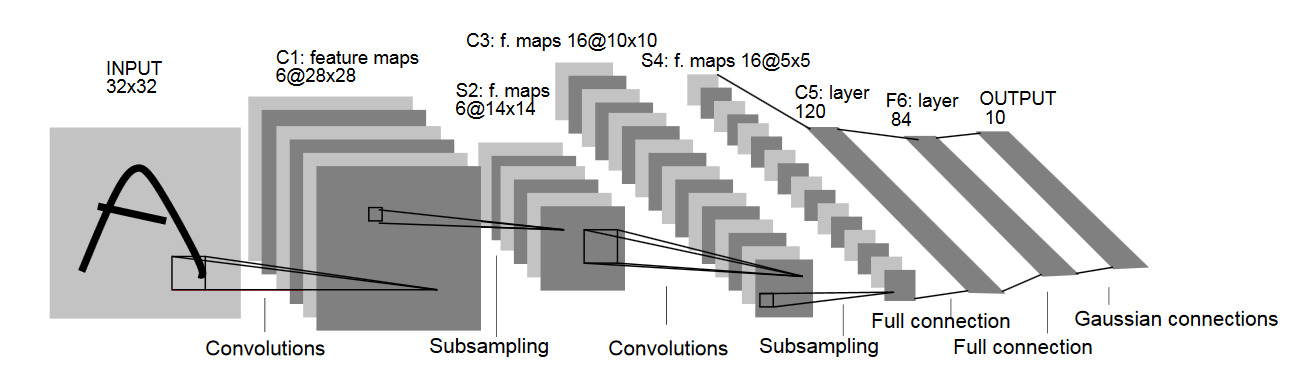
\includegraphics[width=\linewidth]{images/lenet-5.PNG}
    \caption[LeNet-5]{One of the earliest CNN "LeNet-5" used to  recognize handwritten
digits. Image taken from \cite{lecun1998gradient}.}
    \label{fig:lenet-5}
\end{figure}


\subsubsection{Convolution layer}
As the name suggests, convolution layer applies the operation of convolution. This operation should not be confused with convolution in other domains such as signal processing. Unlike fully connected layer (discussed in sec. \ref{sec:fully_connected_layer}), this operation can be applied to any arbitrary sized $m \times n$ matrix. Being a binary operator it accepts two parameters: input matrix $I$ and kernel $K$. The operation can be defined mathematically as:

$$ M(i,j)=(I*K)(i,j)=\sum_m\sum_n I(m,n)K(i-m,j-n)$$

where $I$ is a 2D matrix (a grayscale image) of size $m \times n$ and $K$ is the kernel\cite{goodfellow2016deep}. $(i,j)$ represents the location in output $M$. In computer vision literature, $M$ is also known as feature map. Generally, the size of kernel $K$ is much smaller (usually $3\times 3$) than $I$.

Although the definition looks scary, the convolution operation in practice is quite simple. $M(i,j)$ is simply the sum of element-wise product of sub-matrix of $I$ and $K$. The sub-matrix of $I$ has center at $(i,j)$ and size equal to $K$. Figure \ref{fig:convolution-op} explains the concept in graphical manner for the location $(2,2)$.


\begin{figure}
    \centering
    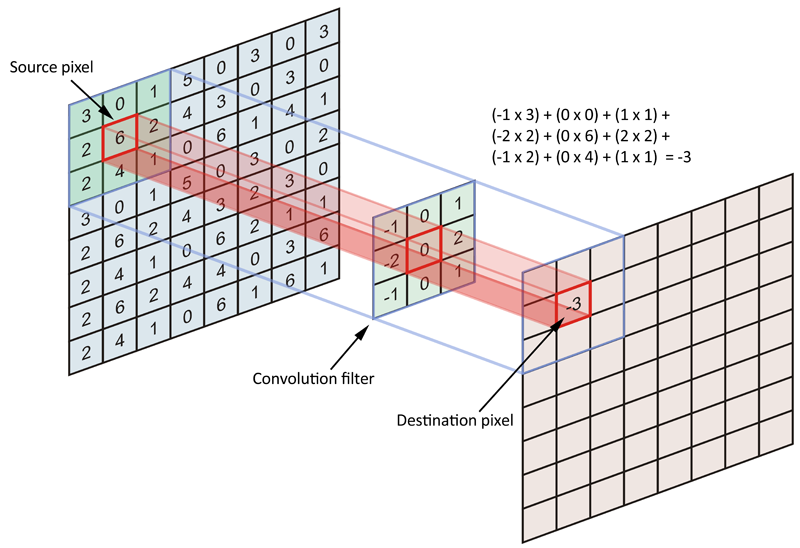
\includegraphics[width=0.8\linewidth]{images/convolution-op.png}
    \caption[Convolution operation]{Convolution operation illustration: destination pixel location is sum of product of kernel weights and corresponding sub-matrix of source matrix. Image taken from \cite{convolution-op}.}
    \label{fig:convolution-op}
\end{figure}

Although the above definition defines 2D convolution, it can simply be extended to 3D as well. In practical architectures, 3D convolution is used. Apart from preserving the grid based image structure, another important aspect of CNN is parameter sharing. In fully connected layer, each parameter of weight matrix is used exactly once while computing the output feature map. On the other hand, when convolution is applied to input image, it generates a feature map which shows how strongly a particular feature occurs at a given location. This parameter sharing nature makes CNN based architecture not only practical but also robust.  

\subsubsection{Activation layer}
A convolution layer is generally followed by a non-linear activation layer. Convolution being a linear operator can only capture linear transformations, therefore a non-linearity is fundamental to learn complicated relationships between input and output. ReLU (\textbf{Re}ctified \textbf{L}inear \textbf{U}nit) function is one of the most widely used non-linearity. It allows a positive input to pass as it is and blocks the negative input. Figure \ref{fig:relu} shows the response of relu function. Other less commonly used non-linearities include TanH ( \textbf{Tan}gent  \textbf{H}yperbolic) and sigmoid functions.

\begin{figure}
    \centering
    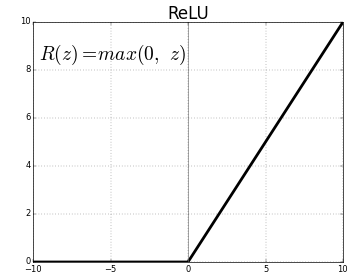
\includegraphics[width=0.7\linewidth]{images/relu.png}
    \caption{ReLU function}
    \label{fig:relu}
\end{figure}


\subsubsection{Pooling layer}
The main goal of pooling layer is to reduce the data dimensionality. It often follows the activation layer. This layer slides a window on input feature map applying a particular pooling operation. This operation is applied on all the values inside the window and can be min, max or average. Based on the operation, it is either called min pooling, max pooling or average pooling. Apart from the window size, another important detail of pooling layer is stride. This parameter refers to no. of pixels sliding window moves forward each time.

Generally stride of the pooling layer is set such that it form non-overlapping windows. For example, applying pooling with $2\times2$ size and a stride of $2$ converts a $14 \times 14$ input feature map to $7 \times 7$. It results into non-overlapping windows as window of size  $2\times2$ moves forward by $2$ pixels every time. On the other hand, if stride is $1$, then every possible window location is visited and windows shall be non-overlapping (if window size is greater than $1$). Figure \ref{fig:pooling} shows an example of max and average pooling.

Pooling can also increase the robustness of feature map by making it \textit{invariant to small translations}\cite{goodfellow2016deep}. Invariance to small translation means that output of pooling layer will not change much even if input experiences a slight translation. This property can be highly desirable as the same object can appear at multiple locations within different images. 

\begin{figure}
    \centering
    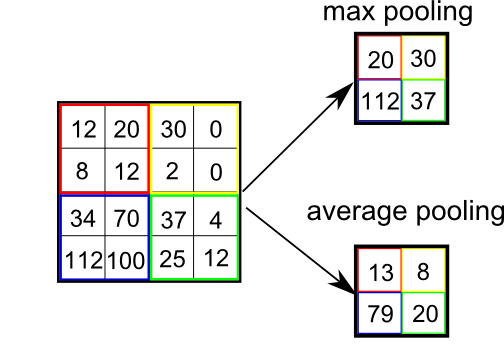
\includegraphics[width=0.7\linewidth]{images/pooling.png}
    \caption[Pooling operation]{An example of max and average pooling applied on feature map of $4\times 4$ size with window size of $2\times 2$ and stride of $2$. Image taken from \cite{ref_pooling}. }
    \label{fig:pooling}
\end{figure}






\subsubsection{Fully connected layer}
\label{sec:fully_connected_layer}
A fully connected layer connects each element of the input feature map to each element of the output feature map. If input and output feature maps contain $m$ and $n$ elements respectively then a fully connected layer has $n \times m$ parameters. Figure \ref{fig:fully_connected} shows a simple fully connected layer. 

A fully connected layer models the input-output relation as an affine linear model. If $f$ and $g$ represent the input and output feature map respectively, then they can be mathematically modeled as 
$$g = Wf+b$$
where $W$ represents the weight parameter matrix and $b$ represents the bias vector. Notice that by the definition of matrix multiplication, $g_i$ is the inner product of $i^{th}$ row of $W$ and $f$. $b_i$ simply adds the bias term. 

This structure can lead to very powerful models, however it is not well suited for images. Even a small $256\times 256$ image can generate a large input feature map of $65536$. This means the size of W shall be $n \times 65536$ where $n$ represents the size of output feature map. Finding the right parameters for such a large $W$ is computationally quite expensive. Further, notice that this layer requires the input feature map $f$ to be a flattened vector. This means that $g$ does not have any spacial interpretation at all. These two reasons make this layer less attractive to generate features for the image data. Never the less, they are still used towards the final stage of model to classify feature maps generated by convolution and pooling layers. 

\begin{figure}
    \centering
    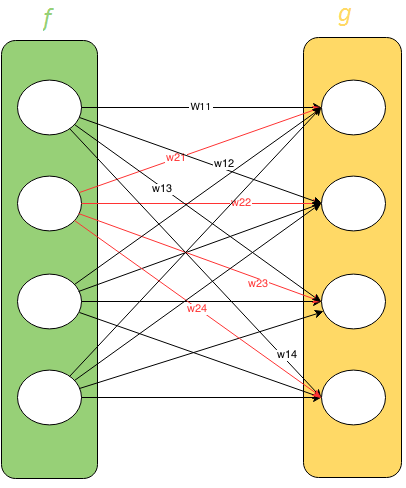
\includegraphics[width=0.5\linewidth]{images/fully_connected.png}
    \caption[Fully connected layer]{Fully connected layer: $f$ represents input feature map and $g$ represents output feature map. Each arrow $Wij$ represents the element connecting $f_i$ to $g_j$. Image taken from \cite{ref_fully_connected}.}
    \label{fig:fully_connected}
\end{figure}

\subsection{Transfer learning}
Transfer learning is a technique in which model weights learnt for one task using one dataset can be used to solve another task on some other dataset. Oquab et. al\cite{oquab2014learning} showed that model weights (for convolutional layers) learnt for object classification using PASCAL VOC dataset\cite{ref_pascal}  could be reused for action classification task. Initial layers of the model learn relatively simpler patters such as horizontal and vertical lines. Deeper layers tend to learn more complicated shapes such as blobs and corners. Learning these layers which can extract these simple features is crucial for any computer vision task. Thus instead of relearning for each task, it makes sense to simply use the pre-learnt model parameters that extract these features. Further, it should be noted that this is useful in both cases where task at hand and dataset are different. This means that weights of a model trained on ImageNet\cite{ref_imagenet} for object classification can be used for object detection on COCO\cite{ref_coco} dataset.  

This technique is particularly useful if dataset is limited. In such a scenario, transfer learning is used in conjunction with fine-tuning. Fine-tuning is closely related with transfer learning. In fine tuning, instead of starting the training with random weights, we start with pre-learnt weights (transfer learning). We take a pre-trained network and chop off the fully connected layer. Now, we attach new fully connected layers and only train these layers while keeping the old convolution layer weights in frozen state. Once the network loss saturates or the model tries to over-fit, we stop the training. Now, we unfreeze the old network weights and restart training. This allows the network to adapt to new data. Since, we are not training the weights of convolution layers from scratch, this is known as fine-tuning.       


\subsection{Object detection}
Problem of object detection refers to detecting objects of certain class (such as person, bird, vehicle etc) at a particular location in an image. Traditionally, sliding window based approach had been used where a window of particular size is slided over the image. Image patch (sub-image covered by the sliding window) is fed  to a feature extractor to produce features such as Harr\cite{vioda2001rapid}, SIFT\cite{lowe1999object} or HoG\cite{lin2008pose}. These features are then fed to a classifier such as fully connected neural network or SVM (Support Vector Machine). This classifier predicts the class labels (object category) whereas the location of sliding window is considered to be the location of predicted object.

However in recent years, significant improvement has been made by switching from hand-crafted features (such as Harr, SIFT and HoG) to CNN based features. One of the initial approaches to solve object detection problem using CNN was Overfeat\cite{sermanet2013overfeat}. Other approaches that successively built upon Overfeat include RCNN\cite{ref_rcnn}, Fast-RCNN\cite{ref_fastrcnn} and Faster-RCNN\cite{ren2015faster}. We shall briefly discuss the approach followed by these methods. 

\subsubsection{Overfeat}
Overfeat\cite{sermanet2013overfeat} was the first paper to propose the use of CNN for object detection on ImageNet\cite{ref_imagenet} dataset. Their approach is simple and straight forward. They slide a window on image and for each window they compute convolutional features. These convolutional features are fed to two separate fully connected sub-networks which predict the label and bounding box for each window respectively. Though this approach significantly improves detection accuracy, it is inherently slow as sliding window generates a lot of patches. Following pseudo code explains their approach.

\begin{lstlisting}[language=Python, caption=Overfeat pseudo code]
for window in windows:
    patch = get_patch(image,window)
    features = compute_conv_features(patch)
    label = classify_label(features)
    bbox = regress_bbox(features)
\end{lstlisting}

\subsubsection{RCNN}
Instead of using sliding window approach Ross Girshick et al.\cite{ref_rcnn} proposed to use a RoI (Region of Interest) based approach. They use selective search\cite{uijlings2013selective_search} to generate category independent RoIs. These RoIs (which are far less in number than sliding windows) are then passed through the same pipeline as Overfeat. The result is significant reduction in time as far less regions needs to be evaluated. 

\begin{lstlisting}[language=Python, caption=RCNN pseudo code]
rois = apply_region_proposal(image)
for roi in rois:
    patch = get_patch(image,roi)
    features = compute_conv_features(patch)
    label = classify_label(features)
    bbox = regress_bbox(features)
\end{lstlisting}

\subsubsection{Fast-RCNN}
Though RCNN showed a significant speedup and improvement in accuracy as compared to Overfeat, it still applied expensive convolutional operation on each RoI independently. This makes it slow in inference as well as in training. Most of the these RoIs are overlapping and thus computational resources are wasted during re-computation of overlapping RoIs.  Fast-RCNN\cite{ref_fastrcnn} circumvents this issues by sharing convolutional features. Convolutional feature extraction process is taken out of the loop and features are computed for the complete image in single step. Later on, features corresponding to each ROI are extracted from the pre-computed feature map. This technique 
makes Fast-RCNN 10x faster than RCNN in training and 150x faster in inference.

One important detail in Fast-RCNN is how we handle RoIs of different sizes. Each RoI has feature size corresponding to its own size. In order to feed the features to fully connected networks (for label and bounding box prediction), these features must be transformed to a particular size.  Fast-RCNN proposes RoI pooling for this purpose. This is similar to Max pooling. However instead of sliding the window on feature map, the whole feature map is converted to a fixed size grid. Max pooling operation is applied on each grid cell and the result has the same size as the size of grid. Following pseudo code explains Fast R-CNN.

\begin{lstlisting}[language=Python, caption=Fast-RCNN pseudo code]

features = compute_conv_features(image)
rois = apply_region_proposal(image)
for roi in rois:
    patch_features = apply_roi_pooling(features,roi)
    label = classify_label(patch_features)
    bbox = regress_bbox(patch_features)
\end{lstlisting}

\subsection{Background subtraction}
Background subtraction is a technique that allows foreground in an image to be extracted. It is a fundamental component in  most conventional (non-deep learning) computer vision pipelines. All the background subtraction techniques depend on some kind of background model. When a new images comes in, it is compared with the existing background model. Those pixels (or regions) which do not fit the background model well are considered to be foreground. Generally, foreground in image is closely related to motion or change. 

We studied a few different background subtraction techniques. SVD\cite{chetverikov2010approximation} and RPCA\cite{candes2011robust} are two well known schemes for background modeling. Thus, they are well suited for background modeling but not for background subtraction/foreground extraction. Furthermore, both of these techniques take an array of frames to develop the background model. They are not flexible enough to update their model to changing scenarios such as change in light. MoG (Mixture of Gaussian)\cite{zivkovic2006efficient} based background subtraction presents itself as a simple and effective method. Due to low computational cost and simplicity, it has very low frame processing time. However, it is highly susceptible to noise.

GSoC(Google Summer of Code) and LSBP(Local SVD Binary Pattern) are two recent background subtraction algorithms. They produce state-of-the art results on foreground segmentation datasets. However, they are extremely slow as compared to MoG. GSoC, however is relatively faster than LSBP.  





\newpage